\documentclass{standalone}
\usepackage{tikz}
\usepackage{ctex,siunitx}
\usepackage{tkz-euclide}
\usepackage{amsmath}
\usetikzlibrary{patterns, calc}
\usetikzlibrary {decorations.pathmorphing, decorations.pathreplacing, decorations.shapes,}
\begin{document}
\small
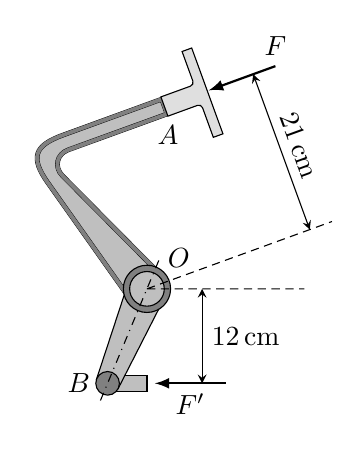
\begin{tikzpicture}[>=latex,scale=1.0]
  \draw[double=gray,line width=0.05mm,double distance=0.5mm,fill=lightgray]( 0.187, 2.409)--
  (-1.068, 1.952)..controls(-1.437, 1.818)and(-1.485, 1.666)..(-1.258, 1.346)--
  (-0.204,-0.144)--
  ( 0.177,0.176)--
  (-1.073,1.436)..controls(-1.183,1.547)and(-1.147,1.711)..(-1.000,1.765)--
  ( 0.256,2.221)--cycle;
  \fill[lightgray,draw=black](-0.5,-1.3)rectangle(0,-1.1);
  \draw[fill=lightgray](-0.2375,0.0781)--(-0.6425,-1.1531)--(-0.3664,-1.2682)--(0.2227,-0.1136)--cycle;
  \fill[gray,draw=black](0,0)circle(0.3);
  \fill[lightgray,draw=black](0,0)circle(0.22)node[above right=2mm,text=black]{$O$};
  \fill[gray,draw=black](-0.5,-1.2)circle(0.15)node[left=1mm,text=black]{$B$};
  \draw[thin,dashdotted](0.15,0.36)--(-0.6,-1.44);
  \draw[thin,densely dashed](0,0)--(2,0)(0,0)--(20:2.5);
  % \draw[lightgray!50,line width=2.6mm](0.2215,2.3154)--++(20:0.6)--++(110:0.6)--++(-70:1.2);
  \draw[fill=lightgray!50](0.2215,2.3154)--++(110:0.13)--++(20:0.4)arc(-70:20:0.05)--++(110:0.4)--++(20:0.13)--++(-70:1.16)--++(200:0.13)--++(110:0.4)arc(20:110:0.05)--++(200:0.4)node[below,text=black]{$A$}--cycle;
  \draw[thick,->]([shift=(110:2.1)]20:2.5)--++(200:0.9)node[at start,above]{$F$};
  \draw[thick,->](1.0,-1.2)--(0.1,-1.2)node[midway,below]{$F'$};
  \draw[thin,stealth-stealth](0.7,-1.2)--(0.7,0)node[midway,right]{\qty{12}{cm}};
  \draw[thin,stealth-stealth](20:2.2)--++(110:2.1)node[midway,sloped,above]{\qty{21}{cm}};
\end{tikzpicture}
\end{document}